\documentclass[12pt]{article}
\usepackage{times,url}
\usepackage{code} 
%\usepackage{proof}
%\usepackage{newcode}
%\usepackage{epsfig}
\usepackage{psfig}

\newcommand{\cut}[1]{}

\newcommand{\appref}[1]{Appendix~\ref{#1}}
\newcommand{\secref}[1]{Section~\ref{#1}}
\newcommand{\tblref}[1]{Table~\ref{#1}}
\newcommand{\figref}[1]{Figure~\ref{#1}}
\newcommand{\listingref}[1]{Listing~\ref{#1}}
%\newcommand{\pref}[1]{{page~\pageref{#1}}}

\newcommand{\eg}{{\em e.g.}}
\newcommand{\cf}{{\em cf.}}
\newcommand{\ie}{{\em i.e.}}
\newcommand{\etc}{{\em etc.\/}}
\newcommand{\naive}{na\"{\i}ve}
\newcommand{\role}{r\^{o}le}
\newcommand{\forte}{{fort\'{e}\/}}
\newcommand{\appr}{\~{}}

\newcommand{\bftt}[1]{{\ttfamily\bfseries{}#1}}
\newcommand{\kw}[1]{\bftt {#1}}
\newcommand{\Pthen}{\kw{Pthen}}
\newcommand{\pads}{\textsc{pads}}
\newcommand{\padsl}{\textsc{padsl}}
\newcommand{\padst}{\textsc{pads/t}}
\newcommand{\datatype}{\textsc{PADS/T}}
%\newcommand{\datatype}{\textsc{DataType}}
\newcommand{\C}{\textsc{C}}
\newcommand{\perl}{\textsc{Perl}}
\newcommand{\ml}{\textsc{ml}}
\newcommand{\sml}{\textsc{sml}}
\newcommand{\smlnj}{\textsc{sml/nj}}
\newcommand{\java}{\textsc{java}}
\newcommand{\ddl}{\textsc{ddl}}
\newcommand{\xml}{\textsc{xml}}
\newcommand{\datascript}{\textsc{DataScript}}
\newcommand{\packettypes}{\textsc{PacketTypes}}
\newcommand{\erlang}{\textsc{Erlang}}

\newcommand{\Core}{Ad hoc}
\newcommand{\core}{ad hoc}
\newcommand{\pvalue}{\core{} value}
\newcommand{\ppat}{\core{} pattern}
\newcommand{\ptype}{\core{} type}

\newcommand{\padsc}{\textsc{pads}/\C{}}
\newcommand{\padsml}{\textsc{pads}/\ml{}}

\newcommand{\dibbler}{Sirius}
\newcommand{\ningaui}{Altair}
\newcommand{\darkstar}{Regulus}

\newcommand{\pdgood}{{\tt G}}
\newcommand{\pdbad}{{\tt B}}
\newcommand{\pdnest}{{\tt N}}
\newcommand{\pdsem}{{\tt S}}
\newcommand{\ptypes}{T}
\newcommand{\patreadpd}[2]{{\tt #1<<#2>>}}
\newcommand{\btm}{\cd{BOT}}


\newcommand{\lsem}{{[\![}}
\newcommand{\rsem}{{]\!]}}


\newcommand{\figHeight}[4]{\begin{figure}[tb]
	\centerline{
	            \epsfig{file=#1,height=#4}}
	\caption{#2}
	\label{#3}
	\end{figure}}

%% Environment for typesetting BNF grammars. Uses display math mode.
\newenvironment{bnf}
     {%% local command definitions:
        %% BNF definition symbol
      \def\->{\rightarrow}
%%      \def\::={{::=} &}
      \def\::={\bnfdef &}
      \def\|{\bnfalt}
      \newcommand{\name}[1]{\text{##1}}
        %% non-terminal
      \newcommand{\nont}[1]{{##1}}
      \newcommand{\meta}[1]{& ##1 &}
      \newcommand{\descr}[1]{& \text{// ##1}}
      \newcommand{\opt}[1]{ [##1] }
      \newcommand{\opnon}[1]{\opt{\nont{##1}}}
      \newcommand{\none}{\epsilon}
      \newcommand{\nwln}{\\ &&&}
      \newcommand{\nlalt}{\\ && \| &}
      \[\begin{array}{lrlll}
     }
     {\end{array}\]}

\newcommand{\mcd}[1]{\mathtt{#1}}
\newcommand{\ppair}[3]{#1{:}#2 \mathrel{**} #3}
\newcommand{\parray}[3]{#1\;\mcd{Parray}(#2,#3)}
\newcommand{\pset}[3]{\{#1{:}#2\,|\,#3\}}
\newcommand{\pstream}[1]{#1\;\mcd{stream}}
\newcommand{\precord}[1]{\{\{#1\}\}}


%%%%%%%%%%%%%%%%%%%%%%%%%%%%%%%%%%%%%%%%%%%%%%%%%%%%%%%%%%%%%%%%%%%%%%%%%%%%
\voffset             0in    %  top vertical offset
\hoffset             0in    %  left horizontal offset
\oddsidemargin       0pt    %  Left margin on odd-numbered pages.
\evensidemargin      0pt    %  Left margin on even-numbered pages.
\topmargin           0pt    %  Nominal distance from top of page to top of
\headheight          0pt    %  Height of box containing running head.
\headsep             0pt    %  Space between running head and text.
\textwidth         6.5in    %  Width of text on page
\textheight          9in    %  Height of text on page
\setlength{\parskip}{.05in}
\renewcommand{\floatpagefraction}{.9}
\renewcommand{\textfraction}{0.1}
% \renewcommand{\baselinestretch}{1.01}
%\input{macro}  %%%  other macro definitions

%%%%%%%%%%%%%%%%%%%%%%%%%%%%%%%%%%%%%%%%%%%%%%%%%%%%%%%%%%%%%%%%%%%%%%%%%%%%
\begin{document}

%\begin{center}
{\bf BAA Number:} BAA 09-029

\vspace{.5in}

{\bf Title of Proposal:}  
Automatic Tool Generation and Monitoring for Networked Applications

\vspace{.5in}

{\bf Identity of prime offerer:}
\begin{quote}
Princeton University \\
Computer Science Department \\
35 Olden St, \\
Princeton, NJ 08540
\end{quote}

\vspace{.5in}

{\bf Technical Contact:}  
\begin{quote}
name \\
tel \\
fax \\
email \\
\end{quote}

\vspace{.5in}

{\bf Administrative contact:}
\begin{quote}
name \\
tel \\
fax \\
email \\
\end{quote}

\vspace{.5in}

{\bf Duration of effort:} 35 months
%\end{center}

\newpage

\setcounter{page}{1}
\pagenumbering{roman}
\appendix
%%%%%%%%%%%%%%%%%%%%%%%%%%%%%%%%%%%%%%%%%%%%%%%%%%%%%%%%%%%%%%%%%%%%%%%%%%%%

% %%%%%%%%%%%%%%%%%%%%%%%%%%%%%%%%%%%%%%%%%%%%%%%%%%%%%%%%%%%%%%%%%%%%%%%%%%%%
\section{Table of Contents}
\tableofcontents\
% \vspace*{.1in} 
% \begin{center}
% {\Large\bf\em{}This is a place-holder. Fastlane generates this page automatically.}
% \end{center} 
\newpage
%%%%%%%%%%%%%%%%%%%%%%%%%%%%%%%%%%%%%%%%%%%%%%%%%%%%%%%%%%%%%%%%%%%%%%%%%%%%
\pagenumbering{arabic}
\setcounter{page}{1}
%%%%%%%%%%%%%%%%%%%%%%%%%%%%%%%%%%%%%%%%%%%%%%%%%%%%%%%%%%%%%%%%%%%%%%%%%%%%

\section{Statement of Work}

%%%%%%%%%%%%%%%%%%%%%%%%%%%%%%
% \centerline{
% \begin{tabular}{cc}
%           \\[-1ex]
% \multicolumn{2}{c}{Automatic Tool Generation for Ad Hoc Scientific Data} \\
%           & \\[-1ex]
% David Walker (PI)\\
% Princeton University\\[2ex]
% \end{tabular}}
%%%%%%%%%%%%%%%%%%%%%%%%%%%%%%

\paragraph*{Intellectual Merits:} 
In every scientific discipline, researchers are digitizing their knowledge and
beginning to use computational methods to categorize,
query, filter, search, diagnose, and visualize their data.  
While this effort is leading to remarkable advances,
it is also generating enormous amounts of {\em ad hoc data}.
Ad hoc data is any data for which standard data processing tools
such as query engines, statistical packages, graphing tools, parsers, printers,
transformers or programming libraries are not readily available.
This data, which is often unpredictable, poorly documented,
filled with errors, high volume and unwieldy,
poses tremendous challenges to its users and the software
that manipulates it.  We cannot maximize the productivity of top 
computational scientists unless we can maximize the efficiency and 
accuracy with which they deal with this data.

Our overall goal is to alleviate the burden, risk and confusion
associated with ad hoc data.  Our overall strategy is (1) to develop a
specification language capable of precisely describing any ad hoc data
format at an easy-to-understand, high level of abstraction and (2) to
automatically generate useful data processing tools including
programming libraries, a query engine, format converters, a
statistical summarizer, a histogram generator and others.
 
We will accomplish our task by building upon our preliminary data
description and processing system, \pads{}, created by the PI and his
collaborators.  This preliminary system demonstrates the basic
feasibility of the \pads{} approach, but there is much research to do.
While the work to date demonstrates the feasibility of the \pads{}
approach, the \pads{} design and implementation are still in their
infancy: We have discovered many common, real-world data formats that
the current PADS infrastructure is incapable of describing, parsing or
analyzing.  To address these deficiencies, we propose to explore
innovative ways of extending the basic \pads{} specification language
and related infrastructure.  The second thrust of our research
involves improving the automatic tool generation infrastructure in the
\pads{} system.  The current tool generation system is brittle,
inflexible and suffers from subpar performance.  We will develop a
novel extension to \pads{} that allows users to augment \pads{}
descriptions with application-specific attributes and customizations.
The attributes convey semantic information to the tool generators and
the customizations improve error-handling and performance.  Our new
architecture has the promise of being substantially more robust,
flexible and efficient.  Finally, in order to improve the reliability
of the infrastructure, we will formalize \pads{} and prove important
correctness properties of our formal model.  Overall, this proposal
involves challenging research in language design, efficient systems
implementation and semantic analysis, all aimed at solving real-world
data processing problems.

\paragraph*{Broader Impacts:}  We are collaborating with Kathleen Fisher
and Mary Fernandez at
AT\&T who will be able to use our tools to address real problems such
as telephone fraud detection.  In addition, our tools will be freely
available to researchers and scientists over the web.  Moreover, part
of our mission will be to work with specific biologists and
physicists at Princeton and the broader community to help them with
their data processing needs.  We have already been meeting with Olga
Troyanskaya, who works in Princeton's Lewis-Sigler Institute for
Integrative Genomics on pathway modeling and analysis of
protein-protein interactions, and with Rachel Mandelbaum, Ph.D. candidate
in physics who analyzes cosmology data.  Many of our proposed extensions to
\pads{} were inspired directly by their data processing needs.  

The collaboration between Computer Science and Genomics will also be an
excellent platform for developing interdisciplinary undergraduate
research projects.  The PI has a proven track-record 
for following through with undergraduate and graduate
educational plans:  Last year, his undergraduate student advisee, Rob Simmons,
won the Princeton Computer Science Senior Thesis Award;
last year and the year before he organized two NSF-sponsored summer schools
on secure and reliable computing.



\section{Technical Approach and Justification}

\section{Introduction}
\label{sec:intro}

{\em Data description languages} are a class of domain specific
languages for specifying {\em ad hoc data formats}, from billing 
records to TCP packets to scientific data sets to server logs.  Examples 
of such languages include 
\bro~\cite{paxson:bro}, \datascript{}~\cite{gpce02}, \demeter~\cite{lieberherr+:class-dictionaries},
\packettypes{}~\cite{sigcomm00}, \padsc{}~\cite{fisher+:pads}, 
\padsml{}~\cite{mandelbaum+:padsml}  and
\xsugar~\cite{xsugar2005}, among others.  All of these languages
generate parsers from data descriptions.  In addition, and unlike
conventional parsing tools such as Lex and Yacc, many also automatically
generate auxiliary tools ranging from printers to \xml{} converters to
visitor libraries to visualization and editor tools.

In previous work, we developed the {\em Data Description Calculus}
(\ddcold{}), a calculus of simple, orthogonal type constructors,
designed to capture the core features of many existing type-based data
description languages~\cite{fisher+:next700ddl,fisher+:ddcjournal}.
This calculus had a multi-part denotational semantics that interpreted
the type constructors as (1) parsers the transform external bit
strings into internal data representations and {\em parse descriptors}
(representations of parser errors), (2) types for the data
representations and parse descriptors, and (3) types for the parsers
as a whole.  We proved that this multi-part semantics was coherent in
the sense that the generated parsers always have the expected types
and generate representations that satisfy an important {\em
canonical forms} lemma.

The \ddcold{} has been very useful already, helping us debug and
improve several aspects of \padsc{}~\cite{fisher+:pads}, and serving
as a guide for the design of \padsml{}~\cite{mandelbaum+:padsml}.
However, this initial work on the \ddcold{} told only a fraction of the
semantic story concerning data description languages.  As mentioned
above, many of these languages not only provide parsers, but
also other tools.  Amongst the most common auxiliary tools
are printers, as reliable communication between programs, either through
the file system or over the Web, depends upon both input (parsing) 
and output (printing).

In this work, we begin to address the limitations of
\ddcold{} by specifying a printing semantics for the
various features of the calculus.  We also
prove a collection of theorems for the new semantics that serve as
duals to our theorems concerning parsing.  This new printing semantics
has many of the same practical benefits as our older parsing 
semantics: We can
use it as a check against the correctness of our printer
implementations and as a guide for the
implementation of future data description languages.  


% First, we extend \ddcold{} with
% abstractions over types, which provides a basis for specifying the
% semantics of \padsml{}. In the process, we also improve upon the
% \ddcold{} theory by making a couple of subtle changes. For example, we
% are able to eliminate the complicated ``contractiveness'' constraint
% from our earlier work. Second, .

% The main practical benefit of the calculus has been as a guide for our
% implementation. Before working through the formal semantics, we
% struggled to disentangle the invariants related to polymorphism. After
% we had defined the calculus, we were able to implement type
% abstractions as \ocaml{} functors in approximately a week.  Our new
% printing semantics was also very important for helping us define and
% check the correctness of our printer implementation.  We hope the
% calculus will serve as a guide for implementations of \pads{} in
% other host languages.  

% In summary, this work makes the following key contributions:
% \begin{itemize}
% \item We simultaneously specify both a parsing and a printing semantics
%   for the \ddc{}, a calculus of polymorphic, dependent types.
% \item We prove that \ddc{} parsers and printers are type safe
%   and well-behaved as defined by a canonical forms theorem.
% \end{itemize}

In this extended abstract, we give an brief overview of the calculus,
it's dual semantics and their properties.  A companion technical
report contains a complete formal
specification~\cite{fisher+:popl-sub-long}.  In comparison to our
previous work on the \ddcold{} at POPL 06~\cite{mandelbaum+:padsml},
the calculus we present here has been streamlined in several subtle,
but useful ways.  It has also been improved through the addition of
polymorphic types.  We call this new polymorphic variant
\ddc{}.  These improvements and extensions, together with
proofs, appear in Mandelbaum's thesis~\cite{mandelbaum:thesis} and in
a recently submitted journal article~\cite{fisher+:ddcjournal}.
This abstract reviews the \ddc{} and extends all the previous 
work with a printing semantics and appropriate theorems.
To be more specific,
sections~\ref{sec:ddc-syntax} through \ref{sec:ddc-sem} present the
extended \ddc{} calculus, focusing on the semantics of polymorphic
types for parsing and the key elements of the printing semantics.
Then, \secref{sec:meta-theory} shows that both parsers and
printers in the \ddc{} are type correct and furthermore that parsers
produce pairs of parsed data and parse descriptors in {\em canonical
  form}, and that printers, given data in canonical form, print
successfully. We briefly discuss related work in \secref{sec:related}, and
conclude in \secref{sec:conc}.

%%% Local Variables: 
%%% mode: latex
%%% TeX-master: "paper"
%%% End: 



\subsection{A Data-Centric Monitor Generation System}

\paragraph*{Basic Architecture}
Figure~\ref{fig:arch} presents the architecture of our proposed
system.  At the top of the picture is the declarative description of all
data that will be used by the monitoring system.  It is here that
programmers encode all their knowledge about their data sources,
including the physical layout of data, its semantic properties
(including constraints on data fields and expected relations
with other fields) so deviations can be flagged as errors, 
its location, access protocol, when the data
will be ready for fetching and how often, etc.

In exchange for the programmer's work in describing their
data sources, the compiler system will generate
a robust and efficient library of {\em format-specific routines} (the center
square in the picture).
The core format-specific 
library includes parser, printer, error detection and data traversal
routines.  The core libraries will also be responsible for controlling
access to and aggregation of any data distributed across wide area
networks and archiving local data along with its description.  

Since these core libraries are compiler-generated from a
high-level data specification, they have many advantages over
hand-written code.  First, the generated code checks
all possible error cases: system errors related to the input file,
buffer, socket, or remote data provider; 
syntax errors related to deviations in the physical
format; and semantic errors in which the data violates user
constraints.  Because these checks appear only in generated code, they
do not clutter the high-level declarative description of the data
source.  Moreover, since tools are generated
automatically by a compiler rather than written by hand, 
they are far more likely to be robust
and far less likely to have dangerous vulnerabilities such as
buffer overflows.  Moreover, as formats change and are updated,
one can make a small change in the high-level description
and the compiler takes care of the rest.  It is extremely unlikely
new vulnerabilities or buffer overflows will be added to the code
base over time as formats change.  Finally, all routines will
be highly optimized for processing the massive
data sets one sees in practice.

In addition to the compiler, which generates the core, format-specific
libraries, the system includes a number of {\em format-independent stubs}
that make use of the generated libraries and implement higher-level
functionality.  Each of these stubs are programmed once, independent
of any format.  In order to implement format-specific behavior, they
are linked with the core libraries, which will be carefully designed to
satisfy a generic, format-independent interface.  Examples of
format-independent tools include a generic query engine that
allows users to extract information from the data, 
a visualization tool that produces
web page summaries of data statistics or a reformatter to convert data
to a new format required by an off-the-shelf tool.  In addition,
a programmer may simply use the generated format-specific libraries directly 
within their own application program, custom built for some unique task. 
Of course whenever a programmer builds a new tool for their application, 
they may do so using the format-independent interface to the generated
libraries.  If they do so, their new tool may be reused by others
who have different data, but require a similar functionality.

At this point, the astute reader may ask why not simply generate
exactly one tool -- a translator that maps the ad hoc data into
XML, a standard format with hundreds of available tools and
rich programming support in all modern, widely used languages.
The problem with such an architecture is that ad hoc formats
are usually quite compact and exploding them into XML representations
can easily result in a space blowup of 8-10 times and an increase
in processing overhead.  Consequently, tiny
sensors in a sensor network cannot afford the expense (processor,
network bandwidth, battery life) of managing
XML data.  More generally, when the data sets get large, and we 
have seen they do in monitoring systems, 
ranging from 100s of MB/week to 100GB/day,
the extra overhead of a 10 times blowup is simply unaffordable.
While compression can reduce this impact, the decompression overheads
of most modern compressors can overwhelm the data processing overhead
of the underlying data.
In an environment where the data is being used and updated
by more than just the monitoring systems, maintaining a parallel
representation in XML is even more painful and impractical.


\subsection{The Prototype Description Language}
To understand further how the \pads{} will be used,
let us look at an example of a simple ad hoc data source:
a tiny fragment of data in the Common Log Format (CLF) that web
servers use to log client requests~\cite{wpp}.  
This ASCII format consists of a sequence of
records, each of which has seven fields: the host name or IP address
of the client making the request, the account associated with the
request on the client side, the name the user provided for
authentication, the time of the request, the actual request, the
\textsc{http} response code, and the number of bytes returned as a
result of the request.  The actual request has three parts: the
request method (\eg, \texttt{GET}, \texttt{PUT}), the requested
\textsc{uri}, and the protocol version.  In addition, the second and
third fields are often recorded only as a '-' character to indicate
the server did not record the actual data.  \figref{figure:clf-records}
shows a couple of typical records.



\begin{figure*}
\begin{footnotesize}
%\begin{center}
\begin{verbatim}
207.136.97.49 - - [15/Oct/1997:18:46:51 -0700] "GET /tk/p.txt HTTP/1.0" 200 30
234.200.68.71 - - [15/Oct/1997:18:53:33 -0700] "GET /tr/img/gift.gif HTTP/1.0" 200 409
240.142.174.15 - - [15/Oct/1997:18:39:25 -0700] "GET /tr/img/wool.gif HTTP/1.0" 404 178
188.168.121.58 - - [16/Oct/1997:12:59:35 -0700] "GET / HTTP/1.0" 200 3082
tj62.aol.com - - [16/Oct/1997:14:32:22 -0700] "POST /spt/dd@grp.org/cfm HTTP/1.0" 200 941
214.201.210.19 ekf - [17/Oct/1997:10:08:23 -0700] "GET /img/new.gif HTTP/1.0" 304 -
\end{verbatim}
\caption{Tiny example of Common Log Format records. }
\label{figure:clf-records}
%\end{center}
\end{footnotesize}
\end{figure*}

With this example, we can examine how to use the prototype 
\pads{} language to describe 
the {\em physical layout} and 
{\em semantic properties} of our ad hoc data source. 
The language provides a type-based model:
basic types describe atomic data such as integers, characters, 
strings, dates, urls, \etc, while
structured types describe compound data built from simpler pieces.

In a bit more detail,
the \pads{} prototype provides a collection of broadly useful base
types.  Examples include 8-bit unsigned integers (\cd{Puint8}), 32-bit
integers (\cd{Pint32}), dates (\cd{Pdate}), strings (\cd{Pstring}),
and IP addresses (\cd{Pip}).  Semantic conditions for such base types
include checking that the resulting number fits in the indicated
space, \ie, 16-bits for \cd{Pint16}.  By themselves, these base types
do not provide sufficient information to allow parsing because they do
not specify how the data is coded, \ie{}, in ASCII, EBCDIC, or binary.
To resolve this ambiguity, \pads{} uses the \textit{ambient} coding,
which the programmer can set.  By default, \pads{} uses ASCII.  
% To
% specify a particular coding, the description writer can select base
% types which indicate the coding to use.  Examples of such types
% include ASCII 32-bit integers (\cd{Pa_int32}), binary bytes
% (\cd{Pb_int8}), and EBCDIC characters (\cd{Pe_char}).  In addition to
% these types, users can define their own base types to specify more
% specialized forms of atomic data.

To describe more complex data, the prototype provides a collection of
structured types loosely based on \C{}'s type structure.  In
particular, the prototype has \kw{Pstruct}s, \kw{Punion}s, and \kw{Parray}s
to describe record-like structures, alternatives, and sequences,
respectively.  \kw{Penum}s describe a fixed collection of literals,
while \kw{Popt}s provide convenient syntax for optional data.  Each of
these types can have an associated predicate that indicates whether a
value calculated from the physical specification is indeed a legal
value for the type.  For example, a predicate might require that two
fields of a \kw{Pstruct} are related or that the elements of a
sequence are in increasing order.  Programmers can specify such
predicates using \pads{} expressions and functions, written using a
\C{}-like syntax.  Finally, \pads{} \kw{Ptypedef}s can be used to
define new types that add further constraints to existing types.

\pads{} types can be parameterized by values.  This mechanism serves
both to reduce the number of base types and to permit the format and
properties of later portions of the data to depend upon earlier
portions.  For example, the base type \cd{Puint_FW(:x:)} specifies
an unsigned integer physically represented by exactly \cd{x}
characters, where \cd{x} is a value that has been read earlier in the
parse.  The type \cd{Pstring(:SPACE:)} describes a string
terminated by a space (when \texttt{SPACE} is defined to be \texttt{' '}).  
Parameters can be used with compound types like arrays and unions to
specify the size of an array or which branch of a union should be
taken.  This parameterization is what makes PADS a {\em dependently-typed}
language and substantially different from languages based on
context-free grammars or regular expressions.

\figref{figure:clf} gives a \pads{} description for the Common Log Format
data.  
We will use this example to illustrate some of the basic
features of the current \pads{} language.  
In \pads{} descriptions, types are declared before they are used, 
so the type that describes the totality of the data source appears 
at the bottom of the description.  
In this case,
the type \texttt{clf\_t}  describes the entirety of the
CLF data source (the \texttt{Psource} type qualifier indicates
this fact explicitly).  

\kw{Pstruct}s describe fixed sequences of data with unrelated types.
In the CLF description, the type declaration for
\cd{version_t} illustrates a simple \kw{Pstruct}. It starts with a 
string literal that matches the constant \cd{HTTP/} in the data source.  It 
then has two unsigned integers recording the major and minor version numbers
separated by the literal character \kw{'.'}.  \pads{} supports character, string,
and regular expression literals, which are interpreted with the ambient character 
encoding. The type \cd{request_t} 
similarly describes the request portion of a CLF record.  In addition
to physical format information, this \kw{Pstruct} includes a semantic constraint
on the \cd{version} field.  Specifically, it requires that obsolete methods
\cd{LINK} and \cd{UNLINK} occur only under HTTP/1.1.  This constraint illustrates
the use of predicate functions and the fact 
that earlier fields are in scope during the processing of later fields, as the 
constraint
refers to both the \cd{meth} and \cd{version} fields in the \kw{Pstruct}.

\kw{Punion}s describe variation in the data format.  For example, the
\cd{client_t} type in the CLF description indicates that the first
field in a CLF record can be either an IP address or a hostname.
During parsing, the branches of a \kw{Punion} are tried in order; the
first branch that parses without error is taken.  The \cd{auth_id_t}
type illustrates the use of a constraint: the branch \cd{unauthorized}
is chosen only if the parsed character is a dash.  \pads{} also
supports a \textit{switched} union that uses a selection expression to
determine the branch to parse.  Typically, this expression depends
upon already-parsed portions of the data source.

\pads{} provides \kw{Parray}s to describe varying-length sequences of
data all with the same type.  The \cd{clf_t} declaration  uses a
\kw{Parray} to indicate that a CLF file is a sequence of \cd{entry\_t}
records.  This particular array terminates when the data source is
exhausted. In general, \pads{} provides a rich
collection of array-termination conditions: reaching a maximum size,
finding a terminating literal (including end-of-record), or satisfying a
user-supplied predicate over the already-parsed portion of the \kw{Parray}. 
\pads{} also has convenient syntax for 
specifying separators that appear between elements of an array and
declaring inter-element constraints including sorting.

The
\kw{Penum} type \cd{method_t} describes a collection of data literals.
During parsing, \pads{} interprets these constants using the ambient
character encoding.  The \kw{Ptypedef} \cd{response_t} describes
possible server response codes in CLF data by adding the constraint
that the three-digit integer must be between 100 and 600.

Finally, the \kw{Precord} annotations deserve comment. It
indicates that the annotated type constitutes a record.  
The notion of a record varies depending upon the data encoding.  
ASCII data typically uses new-line characters to delimit 
records, binary sources tend to have fixed-width records, while 
COBOL sources usually store the length of each record before the actual data.
\pads{} supports each of these encodings of records and allows users to define
their own encodings.  By default, \pads{} assumes records are new-line terminated.
Before parsing, however, the user can direct \pads{} to use a different record
definition.
\texttt{Precords} have error-recovery semantics -- if errors 
in the data cause the parser to become seriously confused,
it will attempt to recover to a record boundary.
In practice, we have found this to be a very robust recovery mechanism
for ad hoc data.  

\begin{figure}
\begin{small}
\begin{code}
\kw{Punion} client\_t \{
  Pip       ip;      /- 135.207.23.32
  Phostname host;    /- www.research.att.com
\};
\mbox{}
\kw{Punion} auth\_id\_t \{
  Pchar unauthorized : unauthorized == '-';
  Pstring(:' ':) id;
\};
\mbox{}
\kw{Pstruct} version\_t \{
  "HTTP/";
  Puint8 major; '.';
  Puint8 minor;
\};
\mbox{}
\kw{Penum} method\_t \{
    GET,    PUT,  POST,  HEAD,
    DELETE, LINK, UNLINK
\};
\mbox{}
bool chkVersion(version\_t v, method\_t m) \{
  \kw{if} ((v.major == 1) && (v.minor == 1)) \kw{return} true;
  \kw{if} ((m == LINK) || (m == UNLINK)) \kw{return} false;
  \kw{return} true;
\};
\mbox{}
\kw{Pstruct} request\_t \{
  '\\"';   method\_t       meth;
  ' ';    Pstring(:' ':) req\_uri;
  ' ';    version\_t      version :
                  chkVersion(version, meth);
  '\\"';
\};
\mbox{}
\kw{Ptypedef} Puint16\_FW(:3:) response\_t :
         response\_t x => \{ 100 <= x && x < 600\};
\mbox{}
\kw{Precord} \kw{Pstruct} entry\_t \{
         client\_t       client;
   ' ';  auth\_id\_t      remoteID;
   ' ';  auth\_id\_t      auth;
   " ["; Pdate(:']':)   date;
   "] "; request\_t      request;
   ' ';  response\_t     response;
   ' ';  Puint32        length;
\};
\mbox{}
\kw{Psource} \kw{Parray} clf\_t \{
  entry\_t [];
\}
\end{code}
\end{small}
\caption{\pads{} description for Web Log data.}
\label{figure:clf}
\end{figure}


\subsection{Monitoring Framework}
\begin{figure*}[t]
\begin{center}
\centerline{\psfig{file=codeen_screen2.ps,width=5in}}
\end{center}
\caption{\label{fig_codeenmon}Screenshot of the CoDeeN monitoring
system, which is the model for our PADS-based system. Rows are
PlanetLab nodes, and most columns contain two data values, with the
column headings indicating the metrics being displayed. The bottom of
the window shows a 2-day history of any cell value. Other windows can
show histories on all nodes for a given metric, or histories of all
metrics for a is agiven node.}
\end{figure*}

To harness the power of PADS and make it easy to use for a variety of
system monitoring tasks, we will implement a generic monitoring
framework capable of scaling from monitoring single feeds at a single
location to monitoring data on thousands of machines in distributed
environments. This framework will consist of the following components:

\begin{enumerate}

\item {\bf Fetch} -- grab the data from one or more sources, in parallel if
needed, and perform whatever aggregation is necessary to begin parsing
the data. While this step may be application-specific, many
applications will use either TCP or UDP combined with a
request/response mechanism. By providing some example code for common
formats, such as HTTP/HTTPS, FTP/SFTP, SCP, SNMP, etc., we can reduce
or eliminate this portion of the ``buy-in'' cost for using our system.
While basic parameterization support will be included, this portion
will obviously be extensible, so that developers can customize it if
needed.

\item {\bf Display} -- once we have the raw data for one or more systems, we
can use the PADS specifications to drive extraction and formatting of
data for display. We will use HTML tables so that the data can be
viewed and manipulated interactively in Web browsers, but will also
support other export formats, such as plain text, CSV (comma-separated
values), tab-delimited format, and, where appropriate, XML
output. Using tables, we can devote one or more rows for each sensor,
machine, or instance, and show multiple data items as columns. In
cases where aggregate representations are appropriate, such as showing
sub-clusters, or multiple machines at a site, we can also show
composite information to summarize more information in the available
screen real estate. Since PADS can also automatically maintain
statistical information about the data it gathers, cell values can be
color-coded automatically, if no additional input is provided by the
developers.

\item {\bf Query} -- using the type information from the PADS description,
provide a mechanism where rows can be selected from the table based on
their contents. Users would be able to provide logical and arithmetic
expressions that could be evaluated using the per-row data, with the
selected rows being shown in the table format, or outputted to one of
the other formats mentioned above. This kind of support can be used to
easily identify sensors/machines behaving strangely, which need some
attention, or have situations of interest. For example, in a Grid
environment, when deploying a new experiment, it may be useful to
select the nodes with lower-than-average utilization.

\item {\bf Archive} -- the data fetched from the machines can be archived
along the with the description to process it. In this way, the data is
self-documenting, and can be accessed in the future using the same
tools as current data. The same support for viewing, querying, etc.,
can be applied to older data, allowing users to easily explore
behaviors over time. Given a reasonably robust description of the data
along with statistical information generated by PADS, it should also
be possible to optimize the on-disk format such that heavily-accessed
data is processed and cached in a post-processed, indexed form, even
if all of the data is stored in a raw format. This optimization can be
transparent to the developer and the users of the tools.

\end{enumerate}

What makes these tasks especially attractive in our context is that
they can be almost entirely automated given a well-formed data
description, making an interactive monitoring tool almost free, given
that the developer provides only slightly more information than is
necessary for parsing. Some of the extra information is entirely
presentational, such as the names used for displaying column headings
on data fields.

To get a sense of how this monitoring system can work, a screenshot of
the custom-built monitor for the CoDeeN content-distribution network
is shown in Figure~\ref{fig_codeenmon}. The entire process was
time-consuming and manual -- the display format and headings for each
row was manually specified, as was the sorting logic. The display
logic for each line was also manually written, to hide irrelevant
fields when nodes are dead or unreachable. Despite the fact that it
was developed for a specific project, it was widely used as a
general-purpose monitoring system for PlanetLab itself. Our proposal
will make generating such systems trivial, and will exploit
optimization opportunities that are time-consuming in
manually-generated systems. More importantly, as the data format
evolves, not only will the monitoring system automatically adapt, but
the archived data will still be available to the monitor, without
requiring multiple versions of the monitoring code for different points
in time.

\subsection{Repository Specifications}
\label{ssec:repo-spec}

Our prototype \pads{} language can describe the syntax and semantic properties
of individual files.  However, diagnosing problems or simply monitoring
the health of applications in networked systems
will usually involve navigating and analyzing {\em sets of files},
not just individual logs.  After all, even individual
applications can generate complex sets of log files.  

As an example, consider the Coral content
distribution system~\cite{coral}, a typical distributed application.
Coral is currently running on PlanetLab system~\cite{planetlab}, a
testbed with 800+ machines distributed world-wide with presence in the
US, Canada, Europe and Asia.  The Coral system periodically collects
four different log files from all machines in its global network.
Coral implementers use this information to understand and debug
it's performance and identify security threats.  They regularly probe the
logs to answer specific questions such as:
\begin{itemize}
\item ``What are 10 the most popular domains and how many requests per 
  domain?'' or
\item ``How many requests were sent by the ten most busy client IPs? (An important signal of misuse)'' or
\item ``How does load look between different nodes?''
\end{itemize}

In order to answer these questions, they have written custom tools
to walk over their repository of log files.  This is a time-consuming and 
error-prone process and their software tools cannot be reused for new 
applications. Moreover, whenever they have new questions to ask, they may
need to write new tools from scratch.

In order to save time, effort, and hence money, we propose to
extend the \pads{} language so that it can describe entire
repositories of application data in a compact, modular fashion.  We
also propose to extend the \pads{} compiler so that it can generate
reuseable interfaces for parsing, traversal, error detection,
transformation and querying of this application data.
To understand how we might extend \pads{} to enable analysis of
entire repositories, let us return to the example of the Coral application, 
mentioned above.  Coral stores it's information in a collection of
log files organized as follows.

\begin{itemize}
\item {\bf Machine Names:}  At the top-level, there is a single directory for
each machine on which a Coral end-point is running.  Hence there are 800+ 
top-level directories.  Each directory
is named using the name of the relevant machine.  
\item {\bf Date-Time:}  Underneith each machine-level directory there is
a set of subdirectories -- one subdirectory for each date (and time) that
monitoring data was acquired.  
\item {\bf Application data:}  Underneith each date-time directory there
are four different kinds of log files:
\begin{itemize}
\item {\bf\tt coralwebsrv.log:}  A log file similar in structure to the log
file fragment presented in Figure~\ref{figure:clf-records} and described in 
Figure~\ref{figure:clf}.
\item {\bf\tt corald.log:}  Logs that describe to which "cluster" of the 
three-level coral hierarchy a node currently belongs, as well as some 
statistics about that nodes' view of the cluster.
\item {\bf\tt coraldnssrv.log:}  Logs of information related to the type of 
DNS query (A, NS, AAAA), the domain being queried, as well as record of 
which A and NS records were returned to that query.
\item {\bf\tt probed.log:}  Logs of traceroutes to clients.
\end{itemize}
\end{itemize}

Figure~\ref{figure:coral-repo} illustrates how we might specify the structure
of the entire repository in an extension of the \pads{} language.  First,
we include a series of single-document descriptions ({\tt corald.pads},
{\tt coraldns.pads}, {\tt coralweb.pads} and {\tt probe.pads}).  These 
included descriptions will be similar to the description shown in
Figure~\ref{figure:clf}.  Next, we begin description of the repository
structure from the bottom up.  The directory specification
called {\tt  host\_info} takes two parameters, {\tt h} and {\tt t}
where {\tt h} is intended to be the associated host and {\tt t} the
associated time the data was collected.  The first two lines of 
{\tt  host\_info} declare {\em logical fields} named {\tt host} and
{\tt time}.  These logical fields are useful for associating meta-data with
specific log files.  The generated interface will provide support for querying
against such generated meta-data.  The following four lines all have the structure:

\begin{code}
<lname> is <filename> as <description> <| <constraints> |>;
\end{code}

The {\tt <lname>} is the logical name of the field.  This logical name
will show up in the generated programmatic interface and may also
serve as a name against which queries may be written.  The 
 {\tt <filename>} component describes the name of the file in the file
system.  Inside {\tt  host\_info} declaration the {\tt <filename>} components
are simple constant strings.  However, they may also be expressed as regular expressions,
or more generally using \pads{} types.  The {\tt <description>} component
provides the name of another description that specifies the structure of the file(s) in question.
Finally, {\tt <constraints>} are used specify any additional information about the
file(s) -- ownership, permissions, creation time, {\em etc.}

The declarations of the {\tt times} directory and the {\tt repository} directory
have a similar structure to the {\tt host\_info} directory.  One difference is that
the {\tt <filename>} component is more sophisticated.  For example, the fragment
{\tt (t:Ptime)} from the {\tt times} directory specification indicates that the
set of file names that match this part of the specification must have a structure
specified by \pads{} type {\tt Ptime}.  Moreover, if a filename does have that structure,
the name will be bound to the variable {\tt t}, which can then be passed as a parameter
to other parts of the description or used in constraints (not shown).

\begin{figure}
\begin{code}
\#include corald.pads     /- imported pads description 
\#include coraldns.pads   /- imported pads description 
\#include coralweb.pads   /- imported pads description 
\#include probe.pads      /- imported pads description 
{\ }
Pdirectory host\_info (h,t) \{
  host = h;
  time = t;
  corald   is  "corald.log"       as corald\_source   <| (perm = "-rwx------") |>;
  coraldns is  "coraldnssrv.log"  as coraldns\_source <| (perm = "-rwx------") |>;
  coralweb is  "coralwebsrv.log"  as coralweb\_source <| (perm = "-rwx------") |>; 
  probe    is  "probed.log"       as probe\_source    <| (perm = "-rwx------") |>;
 \}
{\ }
Pdirectory times (h) \{
  time     is (t:Ptime)           as host_info(h,t)
\}
{\ }
Pdirectory repository \{
   hosts   is (h:Phostname)       as times(h);
\}
\end{code}
\caption{Coral Repository Description}
\label{figure:coral-repo}
\end{figure}

\subsection{Automatic Format Inference}
\label{ssec:format-inference}

When a network problem, compromised machine or malfunctioning application
has been discovered, tracing the problem or attack to
prevent a recurrence is imperative.  This forensic analysis involves
human-guided study of multiple data sources such as log files and
other audit trails.  These data sources are great stores of
information, but they come in many varied and complex forms. They can
contain errors, either unintentional or malicious, and they can be
very, very large.  

To perform forensic analysis, analysts need to quickly understand a
variety of data sources and to ask specific questions about their
contents.  The variety, volume, and complexity of the data mean that
analysts need computational tools to support their analyses and to aid
in information extraction.  However, since every system is different
and the variety of data is so extensive, it is impossible to build
proactively all the specific tools one might need.

In the case of an attack, network forensic analysis should be done in
real-time, perhaps even while an attack is still underway. Not only
does this timeliness increase the chance of discovering the attacker
directly, it also provides the opportunity of identifying and
isolating compromised machines so that the attack cannot spread
further.  Of course, even in the case where an attack or problem is not
deemed urgent, a system adminstrator's time is always valuable --
improvements in administrator efficiency will be translated into 
improvements in their employer's bottom line.

Thus forensic analysts face a twofold problem: (1) they must be able
to ask questions of a wide array of data sources, impossible to
predict in advance, and (2) they must do so highly efficiently.  If
analysts faced only problem (1), they might take their time building
custom tools to query each individual data source from scratch, 
a task that might involve parsing, query support, and visualization 
components.  If analysts faced only problem (2) for a single data source 
known well in advance, they might take the initiative to develop a 
single, standard tool.  Our challenge is to solve both (1) and (2) 
simultaneously: to provide a platform for rapid generation of 
parsing, querying and visualization components for new and evolving
application data sources.

Although PADS descriptions can make managing ad hoc data much easier,
the problem of producing the description in the first place
remains. Writing such descriptions can be tedious and time consuming,
often requiring iteration. First, analysts write a description of as
much of the data as they understand. From this description, they
generate and run analysis tools to find any unknown parts of the
data. They then study those parts and refine the description
accordingly. They repeat this process until all the data either
conforms to the description or constitutes an error in the data rather
than an error in the description.  While the web server log we displayed
earlier may seem easy enough to describe by hand, it is amongst the
simplest examples that we could choose -- application logs may be much
more involved, requiring two-, three- or five-fold more complex descriptions.  
Moreover, the complexity of the situation grows tremendously in a realistic
setting where one must deal with logs of huge size (millions of lines long)
or large archives of logs of many different kinds. 
Having a tool to help produce such descriptions and to generate
data transformation and analysis tools automatically would speed up
forensic analysis and investigation efforts enormously.

\subsubsection*{Format Inference and Tool Generation Architecture}

\begin{figure}
\begin{center}
\centerline{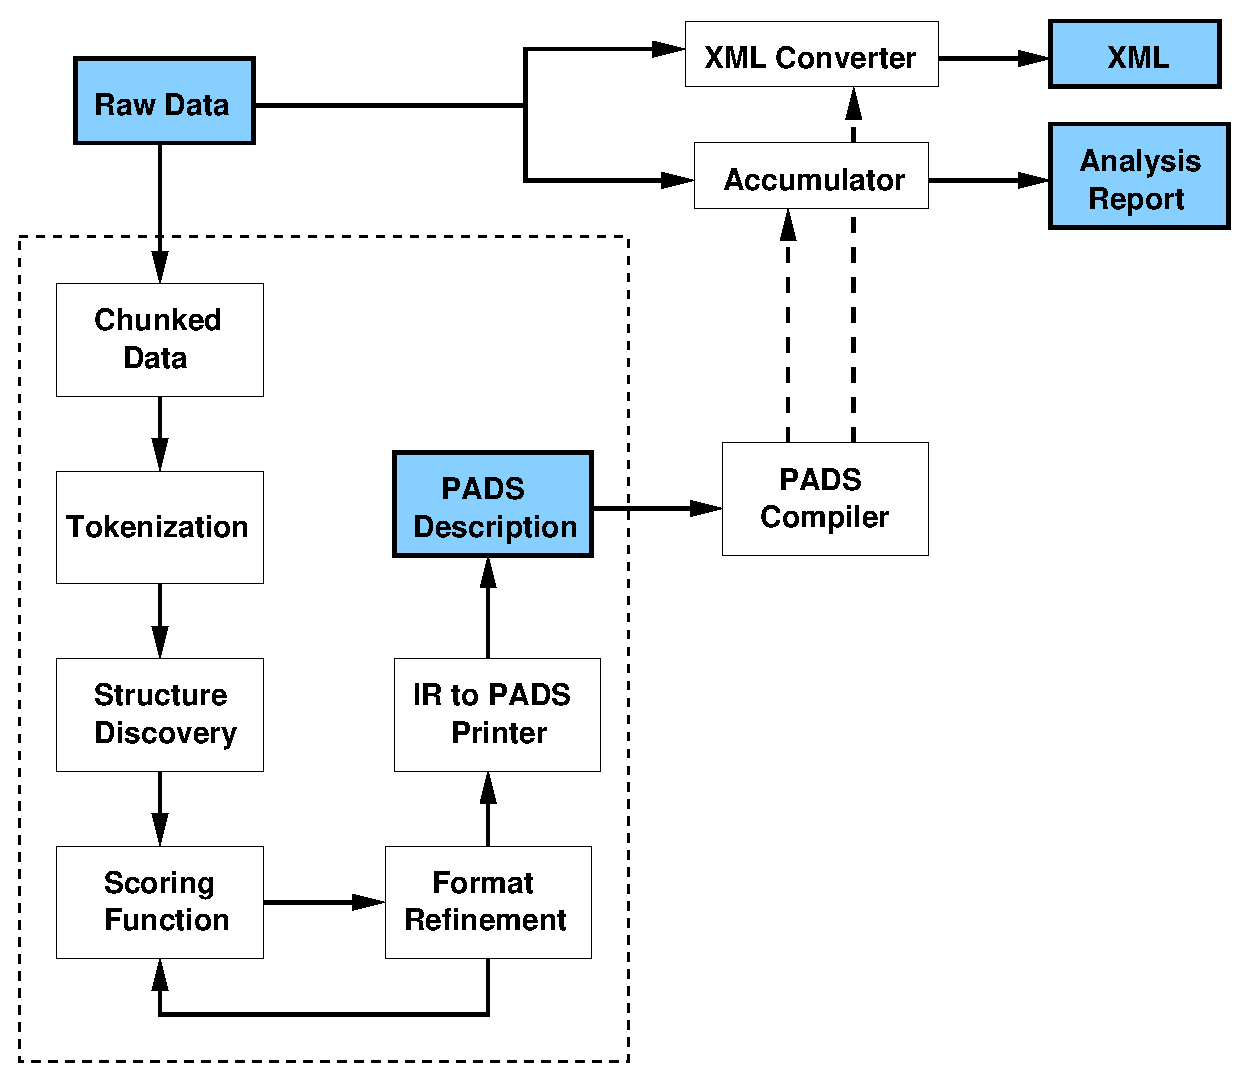
\psfig{file=format-inference-engine.eps,height=2.5in}}
\end{center}
\caption{Modular Architecture of a Format Inference and Tool Generation Engine}
\label{fig:format-inference-engine}
\end{figure}

In preparation for this proposal, we have begun to build a tool for
automatic format inference and data analysis tool generation.  In the
course of building this prototype we have defined a promising, modular 
architecture for solving the problem and performed some preliminary
experiments.  Our experiments have revealed the fact that our proposal
is indeed feasible yet many important challenges must be overcome
to turn our prototype into a robust, precise and viable system.

The overall architecture for the system is presented in
Figure~\ref{fig:format-inference-engine}.  As the diagram shows, the
system takes raw data (sets of systems or application logs) as an
input, pushes the raw data through the inference engine and generates
a \pads{} description.  This description is then automatically fed
through the current \pads{} compiler to produce several simple
data-processing tools including a tool that will read in the data and
translate it to \xml{} as well as a tool (listed in the diagram
as ``the accumulator'')
that will read in the data and output a simple statistical overview
of the data including the distribution of values in each data field and
the number of errors that it finds.

The heart of the system is a highly modular, multi-phase inference 
engine.  We have already begun work on each phase, but also have
many important research questions to answer about each part.
These phases include:

\begin{itemize}
\item {\bf Chunking:}  The first step in the inference process
is to break data into pieces, with the goal that each piece will have
a similar repetitive structure.  Currently, a user can
specify by hand that the data is either chunked line-by-line or file-by-file.
In the future we hope to develop techniques to handle several other
chunking strategies including paragraph-by-paragraph chunking or
directory-by-directory chunking of data sets.  We will develop heuristics
to guess the correct chunking structure when it is unspecified.

\item {\bf Tokenization:}  
The contents of every chunk of data must be divided up
into {\em tokens} such as numbers, words, punctuation, dates, times, 
ip addresses, phone numbers, etc.  Our current prototype includes built-in
support for a small number of basic tokens.  Our experiments indicate
effective tokenization is an extremely important element of the design, yet
astonishingly hard to achieve due ambiguities that arise in token definitions.
In particular, the {\em local} tokenization techniques we are currently using
seem insufficient for disamiguation in general and we are eager to investigate 
techniques that use more {\em global} information to achieve more precise
and useable tokenization.

\item {\bf Structure Discovery:}
After tokenization, the structure discovery phase produces a
candidate format for the data being analyzed.  This candidate is
produced through a recursive divide-and-conquer algorithm that uses
various heuristics to split the data into pieces, analyze the subpieces,
generate formats for subpieces and then combine generated formats to
create an overall description.  This divide-and-conquer algorithm
works well in many cases but occasionally fails, producing \pads{} 
descriptions that do not parse all of the data in the test set.
The reason for this failure is that not all \pads{} features (which
include features from context-free grammars as well as a certain kind
of {\em context-sensitive} grammar) will 
{\em compose} properly with one another.\footnote{Technically, we require
that if $D_1$ and $D_2$ are \pads{} descriptions, then the language of their
concatenation $L(D_1 . D_2)$ must be equivalent to the concatenation
of their languages $L(D_1) . L(D_2)$ and likewise for union and Kleene
closure.  \pads{}, which, for performance reasons, and to handle important
{\em non-context free} features such as dependencies and back references, 
is defined similarly
to the PEGS family of grammars does not have this critical property, 
which is the norm for context-free grammars.}  Hence, in order to overcome
this central problem and develop a robust inference engine, we must
investigate how to redesign several of the core elements of 
the \pads{} language, an interesting theoretical and implementation
challenge.

\item {\bf Scoring Function and Format Rewriting:}
The format generated by the structure discovery is only a rough ``guess''
at the structure of a format.  It is often unnecessarily complicated
in some places and too limited in others.  In order to improve the 
quality of the guess, we score the format and then search for ways
to optimize it using a collection of format rewriting rules.  The
score is based upon the information-theoretic principles embodied in
the Minimum Description Length Principle (MDL)~\cite{mdl}.  In our
experience to date, this format rewriting is somewhat effective --
it reduces the score of the formats initially produced substantially.
However, to the human eye, much improvement can still be made.  We must
investigate the sources of the problems, develop new rewriting rules
and refine the scoring function which guides which rules to apply and
when. 
\end{itemize}

In addition to studying, evaluating, and improving each of the phases
of the inference engine mentioned above, we will engage in two additional
tasks with regards to this element of the grant:

\begin{itemize}
\item {\bf Scaling to large data sets:}
\item {\bf Wholistic repository inference:}
\end{itemize}

\paragraph*{Summary of Format Inference:}  
We have developed a prototype
format inference engine for system log files.  This prototype demonstrates
our ability and the viability of our approach.  However, all phases of
our prototype engine (chunking, tokenization, structure discovery,
scoring and rewriting) must be improved in order to deliver a reliable and
effective automatic tool generation engine.  Moreover, we must develop
completely new algorithms in order to scale our current system up to 
be able to handle application log files of realistic size and complexity.
Finally, we must develop new techniques to extend the scope of our engine
so that it can analyze and uncover the structure
of entire repositories full of log files.

\subsection{Future Naval Relevance}
\label{sec:naval}

Naval information systems involve a complex, heterogeneous
infrastructure with world-wide reach and a vast ecosystem of
interacting, distributed applications. Going forward, as more
information is collected and disseminated to more participants, the
distributed nature of applications will become even more ingrained in
these systems. Given the inherent complexity in distributed systems,
and the difficulty of diagnosing problems in them, monitoring and
proactive detection are necessary to keep this ecosystem functioning
smoothly.  However, as systems and applications diversify, building
appropriate defensive monitoring infrastructure becomes more
difficult, time-consuming, error-prone, and, ultimately, more costly.

We believe that the best hope for building trustworthy, high
reliability systems in such complex future environments is to develop
new technology capable of partially or fully automating the
construction of monitoring software and systems.  Our research will
help proactively find problems, record/archive system status, oversee
operations, debug new applications and detect malicious processes.  In
order to do this, we have proposed a multi-pronged approach that
combines ideas from the programming languages and systems community:

\begin{itemize}
\item Prong 1:  Develop a new programming language capable of specifying the 
form and properties of data produced by networked systems and 
applications.  {\em Automatically} compile those specifications into 
components for parsing, traversal, transformation, error detection,
statistical analysis and querying needed by monitoring systems.

\item Prong 2:  Provide {\em automatic} support for generating the data 
specifications by inferring them directly from available data.

\item Prong 3:  Build new systems support for {\em automatically}
isolating live traffic flows, associating them with their applications,
learning normal behavior, and detecting anomalous traffic.

\item Prong 4:  Wrap all previous components up in a general, scalable,
and adaptive monitoring system capable of
presenting new and evolving data sources to operators and allowing them to
analyze and visualize data across multiple domains.
\end{itemize}

Together, these four prongs form a blueprint for development of the
next generation of monitoring infrastructure.

\section{Project Schedule and Milestones}

\begin{itemize}
\item Year 1:  Re-design of \pads{} specification language and engine
  \begin{itemize}
    \item Design and implement new algorithms for
            the \pads{} engine that will provide the necessary compositionality 
            properties as well as the performance to scale to massive file sizes.
  \end{itemize}
\item Year 1:  Format inference, part 1
  \begin{itemize}
    \item Design, implement new algorithms for the five main phases of the format inference 
      engine: Chunking, tokenization, structure discovery, scoring and format rewriting.
  \end{itemize}
\item Year 1:  Format inference, part 2
  \begin{itemize}
    \item design and implement new incremental inference algorithms that can
      scale to handle log files at least one million lines long.
  \end{itemize}
\item Year 2:  Design of multi-source description language
  \begin{itemize}
    \item extend \pads{} specification language with the capacity to describe
          collections of system and application log files 
  \end{itemize}  
\item Year 3:  Format inference, part 3
  \begin{itemize}
    \item extend format inference engine to enable learning of the structure
       of multi-level, multi-source archives
  \end{itemize}
\end{itemize}

\section{Deliverables}

The main deliverables of this proposal are:

\begin{itemize}
\item The \pads{} domain-specification language and compiler.
\item The \pads{} format inference engine.
\item Comon?
\end{itemize}

\section{Management Approach}

\section{Current and Pending Project and Proposal Submissions}

{\bf CNS 0627650 NSF CT: Well-typed Trustworthy Computing in the 
Presence of Transient Faults \$ 1,100,000 }

\section{Qualifications}

\paragraph*{Kathleen Fisher, Senior Personnel} 
Kathleen Fisher is a senior researcher at AT\&T Labs,
where she has spent the past nine years on projects
related to managing massive amounts of ad hoc network monitoring data.
In the Hancock project~\cite{kdd00,hancock-toplas}, she helped 
design and implement a C-based
domain-specific programming language for processing massive  
transaction streams.  Hancock programs make it easy to build
and maintain profiles of the entities described in such streams. 
AT\&T uses these profiles to monitor networks for fraud 
and to better understand user characteristics.
As the primary architect of the PADS project~\cite{fisher+:pads}, 
Fisher has helped design and implement the prototype PADS
data description language that will form a foundation for the work
described in this proposal.  From PADS descriptions,
a compiler currently produces a parser and a collection of tools for
manipulating the associated data.  

Fisher is an active proponent of increasing the role of women and
minorities in computing and has obtained NSF funding to support
increased involvement of women in computer science (NSF 0243337, ACM
Special Projects: Travel Grants for Faculty at Minority/Female
Institutions to Attend FCRC'03, Co-PI).  This grant was committed to
improving the representation of women and minorities in computer
science. To that end, Fisher and her collaborators 
solicited applications for travel grants from
faculty members at undergraduate institutions with large minority
and/or female enrollments to attend FCRC '03, an umbrella meeting with
16 constituent conferences and many associated workshops and
tutorials.  The organizers of the constituent meetings agreed to waive
the registration fees for all program participants.  Descriptions of
the many meetings that comprised FCRC '03 are available from the FCRC
'03 web site \url{http://www.acm.org/sigs/conferences/fcrc/}.  Fisher
received 56 applications, and was able to award 49 fellowships.

\paragraph*{Vivek Pai, Co-PI} Vivek Pai was partially funded by 
an NSF CAREER award, CCR-0093351, Automatic Retargeting of Network
Servers. He is currently Co-PI on CNS-0520053, An Evolvable
Architecture for Next-Generation Internet Services, and PI on
CNS-0519829 Bridging the 10 GHz / 10 Gbit Gap: Whole-system approaches
for scalable networked services.

His CAREER award led to the enhancement of the Flash Web Server to
support SpecWeb99, an industry-standard benchmark not commonly used in
the academic community due to its complexity. The main result of this
work is an improved research server that is at or near the top of the
results for this benchmark for the classes of hardware tested. In the
process, his group developed new kernel performance debugging tools
that identified numerous performance problems in the FreeBSD operating
system. The modifications they developed to address these problems
have been integrated into FreeBSD and have been shipping for over a
year.  The work also lead to a better understanding of server
performance in SMT (simultaneous multithreading) processors, and why
these processors are not seeing the performance gains in practice that
would have been expected from their simulations.

The two more recent awards have just started, but are already starting
to bear fruit. One recent service developed from this, CoBlitz, is a
scalable large-file transfer service that runs over HTTP. CoBlitz is
now being used by the CiteSeer Scientific Literature Digital Library
to globally deliver electronic copies of research publications. It is
also being used by the Fedora Core Linux distribution in delivering
CD-ISO and DVD-ISO images of their OS distribution.

\paragraph*{David Walker, PI} (NSF CCR-0238328 CAREER: Programming Languages for Secure and Reliable Component Software
Systems, PI)
The goal of Walker's career award is to develop new programming language
technology that will improve the security and reliability of 
component software systems.  More specifically, Walker and his students have 
a new theory of security monitors as formal
automata that transform untrusted applications as they 
execute~\cite{ligatti+:edit-automata}.
This theory allows security
architects to model a variety of different sorts of run-time
enforcement mechanisms, to prove that certain mechanisms can or cannot
enforce various security properties, and to compare the power of
different classes of security monitors~\cite{ligatti+:renewal}.
The theory forms the foundation of an expressive and powerful
program monitoring system for Java~\cite{bauer+:polymer}.

Walker's security monitoring language is a form of 
aspect-oriented programming language.
In order to better understand aspect-oriented technologies and their
potential impact on security, Walker formalized and proved
safe the {\em first} typed, functional and 
aspect-oriented programming language~\cite{walker+:aspects}.
The language has been implemented and
extended with facilities for polymorphic
and type-directed programming~\cite{dantas+:polyaml}.  
Recently, Walker has studied program analysis techniques
that can precisely determine the effect security monitors have on
the code they monitor~\cite{dantas+:harmless-advice,dantas+:harmless-popl}.   
The analysis
can guarantee that a security monitor does not interfere with the 
original application, which greatly increases a user's incentive
to apply security patches.

% To complement his work on run-time monitoring programs, Walker has also
% developed several type systems to ensure basic type and memory safety conditions
% for low-level programs.  Basic type- and memory-safety guarantees provide a foundation on which
% richer security mechanisms can be implemented.  More specifically, he
% has extended his earlier work on typed assembly language (TAL)~\cite{morrisett+:tal,morrisett+:journal-stal} with
% logic-based type systems that can detect memory errors involving
% stack-allocated data~\cite{ahmed+:stack,jia+:stack} and heap or region-allocated
% data~\cite{ahmed+:hierarchical-storage}.  In addition to studying memory safety
% properties, Walker has shown how to use related type-theoretic and logical techniques
% to verify programs~\cite{jia+:ilc} and enforce general software
% protocols~\cite{mandelbaum+:refinements}.  

Walker's career grant also allowed him to be a leader in
programming languages and security education. In 2004 and 2005 he
organized a 10-day summer school on software security and reliable
computing, attended by over 100 participants
combined~\cite{summerschool04,summerschool05}.  Also
in 2005, his undergraduate research advisee, Rob Simmons, won the
Princeton Computer Science Department Senior Thesis Award.
He has recently written a
chapter of a new textbook on typed programming 
languages~\cite{walker:attapl}.

\newpage
%%%%%%%%%%%%%%%%%%%%%%%%%%%%%%%%%%%%%%%%%%%%%%%%%%%%%%%%%%%%%%%%%%%%%%%%%%%%
\section{References Cited}

{\bibliographystyle{abbrv}
\bibliography{pads-long,pads,galax,padsdave,vivek}
}
%{\bibliographystyle{abbrv}
% \small\bibliography{pads}
%} 

\end{document}


